\begin{figure}[t]
  \UseAltLinespread
  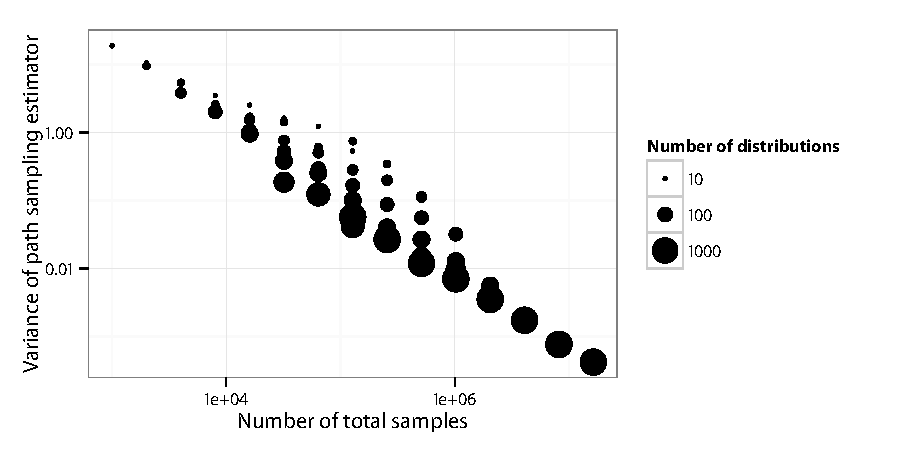
\includegraphics[width=\linewidth]{fig_src/Particle_Iter_Var}
  \caption[Variance of path sampling estimator and total number of samples
  using \protect\smc algorithm]
  {Variance of path sampling estimator and total number of samples using the
    \smc[2] algorithm. Multiple samplers are used to evluate the trade-off
    between the number of particles $N$ and the number of distributions $T$.
    They are configured such that the total number of samples $NT$ is a
    constant. In this figure, the variance of the path sampling estimator from
    100 simulations of each sampler is plotted against the total number of
    samples $NT$ on the log scale. Different configurations of $T$ are
    indicated with different sizes of the dots, larger dots representing
    larger $T$ (and thus smaller $N$). It can be seen that for a particular
    value of $NT$, changing $T$ may change the variance considerably and
    larger $T$ is preferred for most values of $NT$}
  \label{fig:particle iter num}
\end{figure}
